\section{Evaluation}\label{sec:Evaluation}
%Describe the evaluation set up briefly.

% 3 Graph that compares the precision/recall (F1) and time performance of our multiple approaches.


% Our approaches are: 
% 1. Graphs for 2D CNN with simple linear projection on one of the axis.
% 2. 2D CNN with improved transformation from 3D to 2D CNN
% 3. 2D CNN - with - separation and projection and then segmentation with DBSCAN 
% 4. 3D CNN
% 5. Different No. of Layers up to 3 and 2 different size of filter. 


% - We should run it on a standard machine (better on EC2 because it is better reproducible) and show the processing time performance. 


% - We present on our plots, Precision/Recall and Processing time. 


We evaluated our implementation using 5 different settings. 

\begin{enumerate}
  \item 2-Layer CNN on projected data to 2D (Single View) and Object Segmentation with 3D DBSCAN  
  \item 2-Layer CNN on projected data to 2D (Using height projection) and Object Segmentation with 3D DBSCAN
  \item 4-Layer CNN on projected data to 2D (Single View) and Object Segmentation with 3D DBSCAN  
  \item 4-Layer CNN on projected data to 2D (Using height projection) and Object Segmentation with 3D DBSCAN 
\end{enumerate}

Figure \ref{fig:evaluation2} depicts the precision, recall, accuracy and processing time of each of the 4 different experiment settings.  
The figure also includes if in testing all 500 scenes are processed in time or it failed to process them all in the given time limit. 


%\usepackage{graphics} is needed for \includegraphics
\begin{figure*}[htp]
\begin{center}
  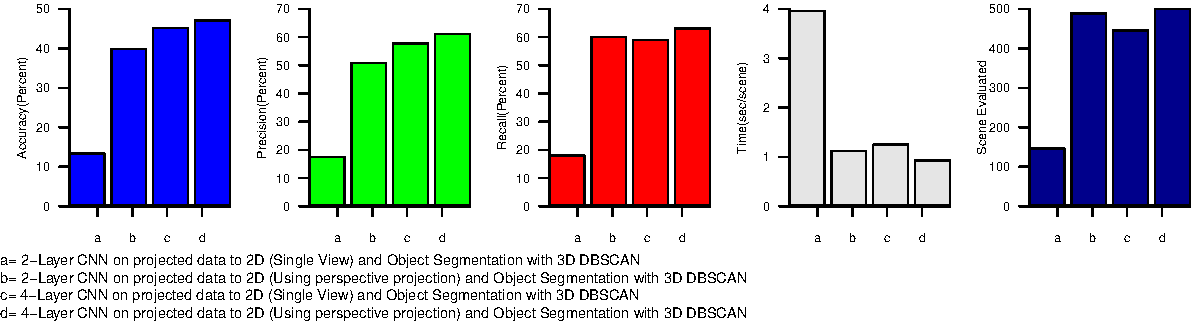
\includegraphics[width=0.6\linewidth]{images/evaluation2.pdf}
  \caption{Precision, Recall, Accuracy and Processing Time of 4 different our Experiment Variation}
  \label{fig:evaluation2}
\end{center}
\end{figure*}


All of the above settings have a data filtering pre-processing step. In Figure \ref{fig:accuracy} and \ref{fig:loss} of our CNN implementation using TensorFlow to classify objects into 28 class types. 


%\usepackage{graphics} is needed for \includegraphics
\begin{figure}[htp]
\begin{center}
        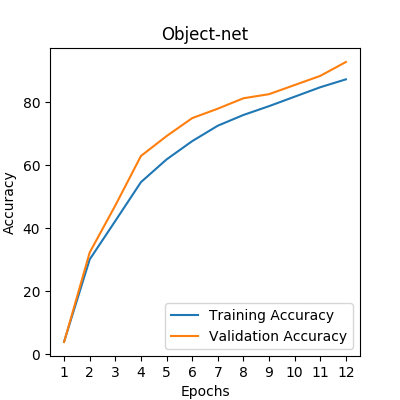
\includegraphics[scale=0.5]{images/accuracy.png}
        \caption{Training and Validation Accuracy}
        \label{fig:accuracy}
\end{center}
\end{figure}



\begin{figure}[htp]
\begin{center}
        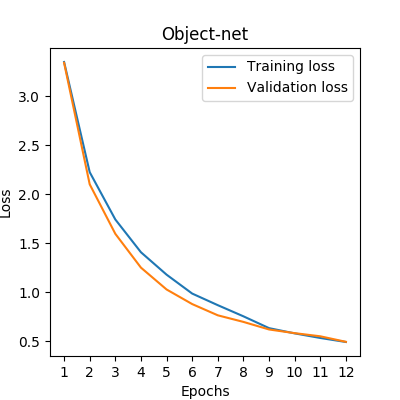
\includegraphics[scale=0.5]{images/loss.png}
        \caption{Training and Validation Loss}
        \label{fig:loss}
\end{center}
\end{figure}

